\documentclass[11pt]{article}

% ----------------------------------------------------------------------
%  Hardware/Software Codesign Proposal
%  Cross-Traffic Intersection Management for Autonomous Vehicles
%  Embedded Electronic Engineering Lab A -- Week 4 milestone
% ----------------------------------------------------------------------

\usepackage[a4paper,top=22mm,bottom=24mm,left=23mm,right=23mm]{geometry}
\usepackage[T1]{fontenc}
\usepackage[expansion=false,protrusion=true]{microtype}
\usepackage{amsmath,amssymb}
\usepackage{booktabs}
\usepackage{array}
\usepackage{xcolor}
\usepackage{enumitem}
\usepackage{caption}
\usepackage{listings}
\usepackage{tikz}
\usetikzlibrary{positioning,arrows.meta,shapes.geometric,fit,backgrounds,calc,decorations.pathreplacing}
\usepackage{titlesec}
\usepackage{fancyhdr}
\usepackage[hidelinks]{hyperref}

% ---------------------------------------------------------------- colours
\definecolor{ink}{HTML}{2B3A42}
\definecolor{swbg}{HTML}{FFF6E3}
\definecolor{hwbg}{HTML}{E9F6EC}
\definecolor{hwgreen}{HTML}{2E7D52}
\definecolor{critbg}{HTML}{FCEDEE}
\definecolor{critred}{HTML}{B23A48}
\definecolor{verbg}{HTML}{F1ECFA}
\definecolor{verpur}{HTML}{6B4E9E}
\definecolor{accent}{HTML}{1F4E79}
\definecolor{neubg}{HTML}{F3F3F3}
\definecolor{shadegray}{HTML}{E6E6E6}
\definecolor{softrule}{HTML}{C9C9C9}

% ---------------------------------------------------------------- inline code
\newcommand{\code}[1]{\texttt{\detokenize{#1}}}

% ---------------------------------------------------------------- section style
\titleformat{\section}{\large\bfseries\color{accent}}{\thesection}{0.65em}{}
\titlespacing*{\section}{0pt}{1.4ex plus .3ex}{0.7ex}
\titleformat{\subsection}{\normalsize\bfseries\color{ink}}{\thesubsection}{0.6em}{}
\titlespacing*{\subsection}{0pt}{1.0ex plus .2ex}{0.4ex}

% ---------------------------------------------------------------- caption style
\captionsetup{font=small,labelfont={bf,color=accent},labelsep=period,skip=5pt}

% ---------------------------------------------------------------- header/footer
\pagestyle{fancy}
\fancyhf{}
\fancyfoot[L]{\footnotesize\color{ink!70}Embedded Electronic Engineering Lab A\,$\cdot$\,Team A --- Group 01}
\fancyfoot[R]{\footnotesize\color{ink!70}\thepage}
\renewcommand{\headrulewidth}{0pt}
\renewcommand{\footrulewidth}{0.4pt}
\renewcommand{\footrule}{\hbox to\headwidth{\color{softrule}\leaders\hrule height \footrulewidth\hfill}}

% ---------------------------------------------------------------- listings
\lstdefinestyle{ccode}{
  language=C,
  basicstyle=\ttfamily\small,
  keywordstyle=\color{accent}\bfseries,
  commentstyle=\color{hwgreen}\itshape,
  numbers=none,
  showstringspaces=false,
  breaklines=true,
  frame=single,
  rulecolor=\color{softrule},
  framesep=7pt,
  backgroundcolor=\color{neubg},
  xleftmargin=2pt,xrightmargin=2pt,
  aboveskip=9pt,belowskip=5pt,
  morekeywords={bool,true,false}
}

% ---------------------------------------------------------------- tikz styles
\tikzset{
  blk/.style={draw=ink,rounded corners=3pt,align=center,font=\footnotesize,inner sep=5pt,line width=0.6pt,minimum height=8mm},
  swblk/.style={blk,fill=swbg},
  hwblk/.style={blk,fill=hwbg},
  critblk/.style={blk,fill=critbg,draw=critred,line width=0.7pt},
  neu/.style={blk,fill=neubg},
  flow/.style={-{Latex[length=2.4mm,width=1.8mm]},line width=0.9pt,draw=accent},
  flowred/.style={-{Latex[length=2.4mm,width=1.8mm]},line width=0.9pt,draw=critred},
  hdr/.style={font=\bfseries\small},
  sub/.style={font=\scriptsize\itshape,text=ink!55},
}

\setlist[itemize]{leftmargin=1.45em,topsep=2pt,itemsep=2.5pt,parsep=0pt}
\renewcommand{\arraystretch}{1.15}

% ---------------------------------------------------------------- line breaking
% absorb long unbreakable inline-code identifiers without breaking them
\tolerance=1200
\emergencystretch=3em

% ---------------------------------------------------------------- float spacing
\setlength{\intextsep}{9pt plus 2pt minus 2pt}
\setlength{\textfloatsep}{10pt plus 2pt minus 2pt}
\setlength{\abovecaptionskip}{4pt}

% ======================================================================
\begin{document}

% ------------------------------------------------------------ title block
\begin{center}
{\color{softrule}\rule{\textwidth}{0.4pt}}\\[1.0ex]
{\LARGE\bfseries\color{ink} Hardware/Software Codesign Proposal}\\[0.7ex]
{\large\bfseries\color{accent} Cross-Traffic Intersection Management for Autonomous Vehicles}\\[1.1ex]
{\normalsize Embedded Electronic Engineering Lab A\;\textbf{$\cdot$}\; Week 4 Milestone}\\[0.6ex]
{\small Prof.\ Dr.\ Achim Rettberg\quad$\cdot$\quad Prof.\ Dr.\ Stefan Henkler}\\[0.3ex]
{\small Team A\;$\cdot$\;Group 01}\\[1.0ex]
{\color{softrule}\rule{\textwidth}{0.4pt}}
\end{center}
\vspace{0.4ex}

% ------------------------------------------------------------ abstract box
\begin{center}
\colorbox{accent!7}{%
\begin{minipage}{0.96\textwidth}
\small
\textbf{\color{accent}Summary.}\; This document is the Week~4 deliverable: a proposal for partitioning the
Road-Side-Unit (RSU) intersection controller between software and hardware, in preparation for the
Week~5 implementation in FreeRTOS and ModelSim. The proposal builds on two artefacts that already
exist and agree with each other --- the UPPAAL timed-automata model verified in Week~2 and the
deterministic C core written in Week~3. Because both already exist, the partition is
\emph{behaviour-preserving by construction}: it changes only \emph{where} each function runs, not the
verified safety contract. The control-dominated scheduling and messaging logic stays in software; the
regular, data-parallel and safety-relevant conflict checking moves into a small hardware
\emph{Conflict \& Safety Coprocessor} that returns one \code{safe_to_grant} bit and runs an independent
collision monitor. The result is a grant decision with constant, easy-to-bound timing, a second
hardware check of the \code{A[] noCollision()} invariant, and a fairness (aging) term that removes the
V5 starvation observed in Week~3.
\end{minipage}}
\end{center}
\vspace{0.6ex}

% ======================================================================
\section{Objective of Week 4}
The course plan splits the project into weekly milestones. Week~3 delivered the first abstract
implementation; Week~4 asks for a \emph{proposal} for the hardware/software codesign; and Week~5 is the
codesign implementation itself, with software in FreeRTOS and hardware in ModelSim. This document is the
Week~4 proposal. It describes how we intend to split the RSU controller and what the interface between
the two sides looks like, so that Week~5 becomes an implementation task rather than a redesign.

The proposal rests on two things we already have: the verified UPPAAL model
(\texttt{\small RSU\_MM1\_\allowbreak MM2\_\allowbreak priority\_\allowbreak emergency\_\allowbreak intersection}) and the deterministic C
core. Since both already
exist and produce the same behaviour, the partition does not alter the fleet, the priority order, the
conflict rules, or the safety queries. It only decides the execution target of each part. The remainder
of the document recaps the verified baseline, states the partitioning criterion, presents the proposed
software and hardware parts together with their register interface, adds the fairness term that the
Week~3 results showed we need, and closes with a verification plan, a construct-by-construct mapping,
and a Week~5 work plan with risks.

% ======================================================================
\section{The Verified Baseline (Weeks 1--3)}
Week~1 fixed the functional requirements: the RSU must serialise conflicting movements, give priority
to emergency and main-street traffic, support both M/M/1 and M/M/2 service, and communicate using only
V2I, I2V and V2V messages. Week~2 turned this into a UPPAAL network of timed automata with two
templates --- \textsf{Vehicle} and \textsf{RSU\_Controller} --- instantiated as one RSU and six
vehicles, and six queries were checked and all hold. Week~3 re-implemented the same model as a
single-threaded, deterministic C program and re-checked the safety invariants at run time.

The geometry and the contract are unchanged. The main street runs \textbf{EAST--WEST} and the side
street \textbf{NORTH--SOUTH}, with the RSU owning the conflict zone. M/M/1 lets one vehicle cross at a
time; M/M/2 lets two cross if they do not conflict, selected by \code{MM_MODE}. Priority is
\emph{emergency $\to$ main street $\to$ side street}, and a right turn is taken before a left turn inside
a conflict. The critical pair is \textbf{V4} (North, right turn) and \textbf{V5} (South, left turn),
which must never cross together; in UPPAAL this is \code{A[] not (crossing[4] && crossing[5])}.
Table~\ref{tab:fleet} lists the exact fleet that was verified.

\begin{table}[h]
\centering
\caption{The verified six-vehicle fleet (as instantiated in the UPPAAL \code{system} block).}
\label{tab:fleet}
\small
\begin{tabular}{@{}llccccl@{}}
\toprule
\textbf{Veh.} & \textbf{Origin} & \textbf{Turn} & \textbf{Emerg.} & \textbf{Period} & \textbf{Cross} & \textbf{Role} \\
\midrule
V0 & EAST  & STRAIGHT & yes & 30 & 4 & Emergency vehicle (main street) \\
V1 & EAST  & STRAIGHT & no & 6  & 5 & Main-street, used for the M/M/2 overlap \\
V2 & WEST  & STRAIGHT & no & 8  & 5 & Main-street, opposite direction \\
V3 & NORTH & STRAIGHT & no & 10 & 5 & Side-street straight \\
V4 & NORTH & RIGHT    & no & 12 & 5 & Critical right-turn vehicle \\
V5 & SOUTH & LEFT     & no & 12 & 5 & Critical left-turn vehicle \\
\bottomrule
\end{tabular}
\end{table}

\noindent
Week~3 also surfaced one problem that this proposal must address. Under strict static priority with
continuous arrivals, \textbf{V5 is never served}, even when the run is extended to 400 ticks. This is
not a modelling bug: the UPPAAL queries check safety and reachability, not liveness, so nothing forbids
it. With the priority encoding in the model, \code{priorityValue} gives
$\text{V0}{=}0 < \text{V1}{=}\text{V2}{=}11 < \text{V4}{=}20 < \text{V3}{=}21 < \text{V5}{=}22$, so V5 sits
at the strict bottom of every tie-break and can be perpetually overtaken. Section~\ref{sec:aging}
fixes this with an aging term in software.

% ======================================================================
\section{Codesign Methodology and Partitioning Criterion}
We follow the standard codesign flow from the module: start from the reference implementation, sort each
function by \emph{how it computes}, then place the work accordingly. The criterion is a single rule:

\begin{center}
\colorbox{neubg}{%
\begin{minipage}{0.96\textwidth}
\small\centering
\textbf{Regular, parallel and timing-critical} work $\to$ \textbf{hardware}.\qquad
\textbf{Irregular, control-heavy and often-changed} work $\to$ \textbf{software}.
\end{minipage}}
\end{center}

\noindent
Applied to the Week~3 functions, the split is clear-cut.

\subsection{Functions that stay in software}
The scheduler loop, the V2I/I2V/V2V message handling, and the state updates \code{requestVehicle()},
\code{grantVehicle()} and \code{finishVehicle()} are sequential, branch-heavy, and tied to the
per-vehicle timers for \code{period} and \code{crossTime}. The priority functions
\code{priorityValue()}, \code{betterPriority()}, \code{existsBetterGrantable()} and
\code{emergencyWaiting()} decide the order of service and are exactly the parts we are most likely to
change later --- for example when adding aging. All of this maps naturally onto FreeRTOS tasks and
queues and stays in software.

\subsection{Functions that move to hardware}
The conflict checking is different in kind. \code{conflict(a,b)}, \code{conflictsWithCrossing(i)} and
\code{noCollision()} are pure functions of the current \code{origin[]}, \code{turn[]},
\code{emergency[]} and \code{crossing[]} values. They hold no state of their own and use no timers. In
software they are also the most repeated work on the decision path:
\begin{itemize}
  \item \code{noCollision()} is an $O(N^2)$ double loop --- $15$ pairwise \code{conflict()} checks for
  $N=6$ --- and it runs on every tick as the safety monitor.
  \item \code{conflictsWithCrossing(i)} is an $O(N)$ scan, and the capacity test calls it for every
  candidate the RSU examines during a grant.
\end{itemize}
In hardware these $15$ pairwise checks all evaluate in parallel in a single clock cycle, so the timing
is constant and easy to bound, and the CPU stops spending cycles on them. The same combinational block
keeps running every clock against the live \code{crossing[]} set, giving an independent hardware check
of the \code{A[] noCollision()} invariant. That dual benefit --- it helps both \emph{timing} and
\emph{safety} --- is the main reason this part belongs in hardware. Figure~\ref{fig:partition} shows the
proposed partition, and Figure~\ref{fig:grant} shows why this kernel dominates a single grant decision.

% ======================================================================
\section{Proposed System Architecture}

% ----------------------------------------------------------- FIGURE 1
\begin{figure}[h]
\centering
\resizebox{\textwidth}{!}{%
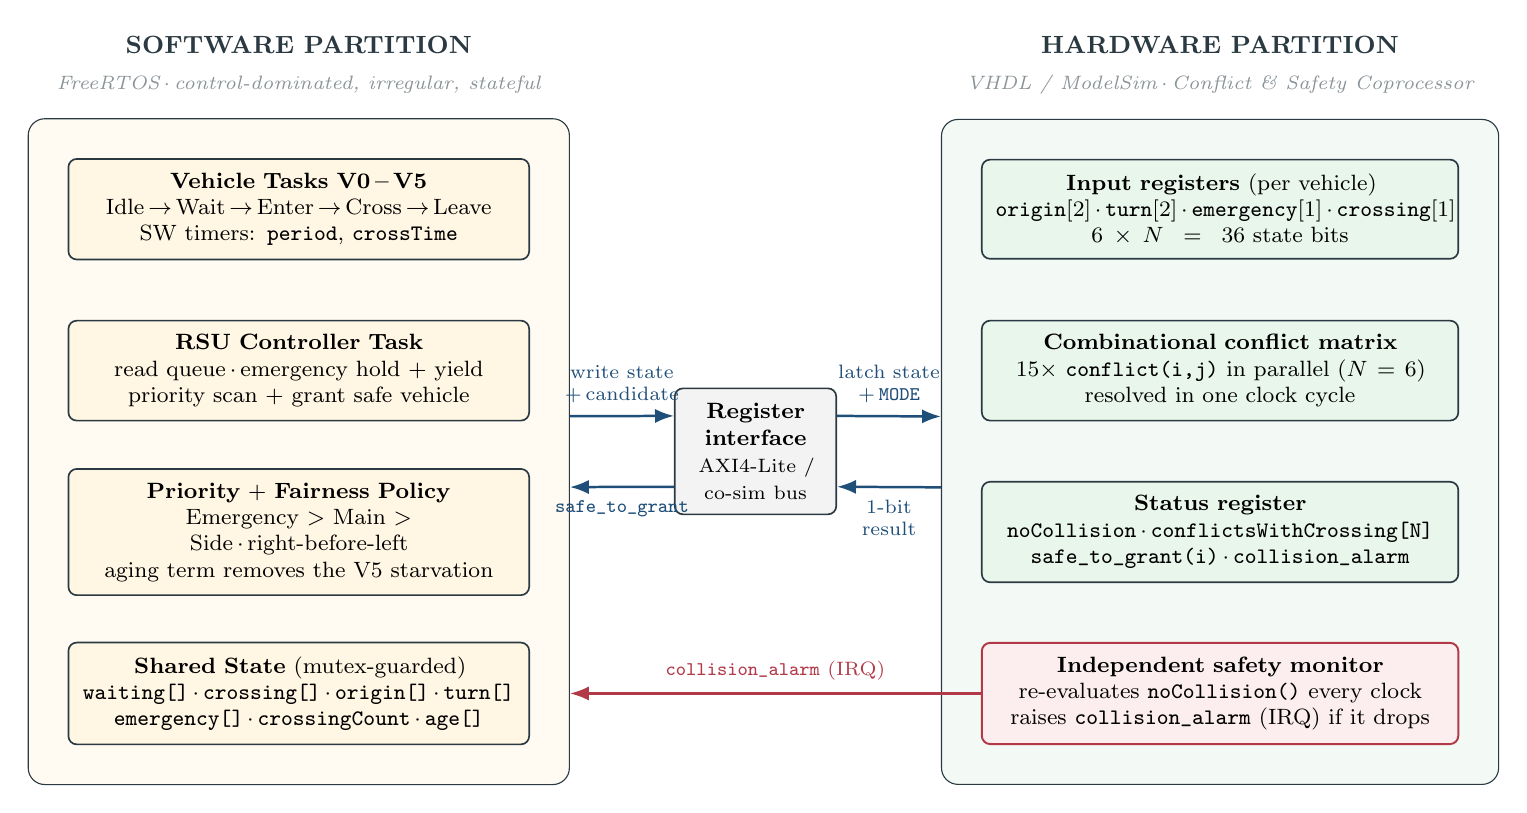
\begin{tikzpicture}[font=\footnotesize]

% ==== software column (centre x = 3.0) ====
\node[swblk,text width=5.5cm] (swA) at (3.0,8.7)
  {\textbf{Vehicle Tasks V0\,--\,V5}\\ Idle\,$\to$\,Wait\,$\to$\,Enter\,$\to$\,Cross\,$\to$\,Leave\\
   SW timers: \code{period}, \code{crossTime}};
\node[swblk,text width=5.5cm] (swB) at (3.0,6.65)
  {\textbf{RSU Controller Task}\\ read queue\,$\cdot$\,emergency hold $+$ yield\\
   priority scan $+$ grant safe vehicle};
\node[swblk,text width=5.5cm] (swC) at (3.0,4.6)
  {\textbf{Priority $+$ Fairness Policy}\\ Emergency $>$ Main $>$ Side\,$\cdot$\,right-before-left\\
   aging term removes the V5 starvation};
\node[swblk,text width=5.5cm] (swD) at (3.0,2.55)
  {\textbf{Shared State} (mutex-guarded)\\ \code{waiting[]}\,$\cdot$\,\code{crossing[]}\,$\cdot$\,\code{origin[]}\,$\cdot$\,\code{turn[]}\\
   \code{emergency[]}\,$\cdot$\,\code{crossingCount}\,$\cdot$\,\code{age[]}};

% ==== hardware column (centre x = 14.7) ====
\node[hwblk,text width=5.7cm] (hwIn) at (14.7,8.7)
  {\textbf{Input registers} (per vehicle)\\ \code{origin}[2]\,$\cdot$\,\code{turn}[2]\,$\cdot$\,\code{emergency}[1]\,$\cdot$\,\code{crossing}[1]\\
   $6\times N = 36$ state bits};
\node[hwblk,text width=5.7cm] (hwMat) at (14.7,6.65)
  {\textbf{Combinational conflict matrix}\\ $15\times$ \code{conflict(i,j)} in parallel ($N=6$)\\
   resolved in one clock cycle};
\node[hwblk,text width=5.7cm] (hwOut) at (14.7,4.6)
  {\textbf{Status register}\\ \code{noCollision}\,$\cdot$\,\code{conflictsWithCrossing[N]}\\
   \code{safe_to_grant(i)}\,$\cdot$\,\code{collision_alarm}};
\node[critblk,text width=5.7cm] (hwMon) at (14.7,2.55)
  {\textbf{Independent safety monitor}\\ re-evaluates \code{noCollision()} every clock\\
   raises \code{collision_alarm} (IRQ) if it drops};

% ==== interface node (centre) ====
\node[neu,text width=1.7cm,minimum height=16mm,align=center] (IF) at (8.8,5.625)
  {\textbf{Register}\\\textbf{interface}\\[2pt]{\scriptsize AXI4-Lite /\\ co-sim bus}};

% ==== containers (one per side) ====
\begin{scope}[on background layer]
  \node[draw=ink,rounded corners=6pt,fill=swbg!45,fit=(swA)(swB)(swC)(swD),inner sep=5mm] (SWBOX) {};
  \node[draw=ink,rounded corners=6pt,fill=hwbg!55,fit=(hwIn)(hwMat)(hwOut)(hwMon),inner sep=5mm] (HWBOX) {};
\end{scope}

% ==== headers (clear of the containers) ====
\node[hdr,text=ink]  at (3.0,10.78)  {SOFTWARE PARTITION};
\node[sub]           at (3.0,10.28)  {FreeRTOS\,$\cdot$\,control-dominated, irregular, stateful};
\node[hdr,text=ink]  at (14.7,10.78) {HARDWARE PARTITION};
\node[sub]           at (14.7,10.28) {VHDL / ModelSim\,$\cdot$\,Conflict \& Safety Coprocessor};

% ==== write lane (top): SW -> IF -> HW ====
\draw[flow] ([yshift=4.5mm]SWBOX.east) -- ([yshift=4.5mm]IF.west)
  node[midway,above=1pt,font=\scriptsize,text=accent,align=center]{write state\\$+$\,candidate};
\draw[flow] ([yshift=4.5mm]IF.east) -- ([yshift=4.5mm]HWBOX.west)
  node[midway,above=1pt,font=\scriptsize,text=accent,align=center]{latch state\\$+$\,\code{MODE}};

% ==== read lane (bottom): HW -> IF -> SW ====
\draw[flow] ([yshift=-4.5mm]HWBOX.west) -- ([yshift=-4.5mm]IF.east)
  node[midway,below=1pt,font=\scriptsize,text=accent,align=center]{1-bit\\result};
\draw[flow] ([yshift=-4.5mm]IF.west) -- ([yshift=-4.5mm]SWBOX.east)
  node[midway,below=1pt,font=\scriptsize,text=accent]{\code{safe_to_grant}};

% ==== alarm lane: monitor -> SW (independent IRQ) ====
\draw[flowred] (hwMon.west) -- (SWBOX.east|-hwMon.west)
  node[midway,above=1pt,font=\scriptsize,text=critred]{\code{collision_alarm} (IRQ)};

\end{tikzpicture}}
\caption{Proposed HW/SW codesign partition. The software side (FreeRTOS) keeps the admission and
scheduling logic, the messages and the queue state; the hardware side (VHDL/ModelSim) holds the
\emph{Conflict \& Safety Coprocessor}, which returns one \code{safe_to_grant} bit per candidate and runs
an independent collision monitor wired to an interrupt.}
\label{fig:partition}
\end{figure}

\subsection{Software part (FreeRTOS)}
\begin{itemize}
  \item \textbf{Vehicle tasks (V0--V5)}: one task each, running the Vehicle FSM from UPPAAL
  (\textsf{Idle, WaitingInQueue, V2V\_Enter, Crossing, V2V\_Leave}). The clock \code{x[i]} becomes a
  FreeRTOS software timer / \code{vTaskDelay} for \code{period} and \code{crossTime}; the committed
  enter and leave steps remain zero-delay transitions.
  \item \textbf{RSU controller task}: reads the requests, runs the priority scan and the grant loop,
  sends the grants and the emergency yield, and owns the queue state. Instead of computing the
  conflicts itself, it queries the coprocessor.
  \item \textbf{Communication}: the channels \code{req[]}, \code{emg_req[]}, \code{grant[]},
  \code{leave[]}, \code{i2v_yield}, \code{v2v_enter} and \code{v2v_leave} become FreeRTOS message
  queues; the broadcast channels are handled as one-to-many task notifications.
  \item \textbf{Shared state}: \code{waiting[N]}, \code{crossing[N]}, \code{origin[N]}, \code{turn[N]},
  \code{emergency[N]}, \code{crossingCount} and \code{emergencyNotified}, guarded by a mutex and mirrored
  into the coprocessor input registers immediately before each decision.
\end{itemize}

\subsection{Hardware part (VHDL / ModelSim): the Conflict \& Safety Coprocessor}
This is a combinational module with a small register interface that resolves the conflict relation for
the whole fleet at once.
\begin{itemize}
  \item \textbf{Inputs (registered)}: \code{origin} (2 bits), \code{turn} (2 bits), \code{emergency}
  (1 bit) and \code{crossing} (1 bit) per vehicle --- $6$ bits $\times\,N = 36$ bits of state.
  \item \textbf{Conflict matrix}: $15$ \code{conflict(i,j)} cells in parallel, each a small Boolean
  expression over \code{isMainRoad}, \code{oppositeDirection}, the same-origin case and the turn rules.
  This is a direct translation of the C \code{conflict()} function into logic.
  \item \textbf{Outputs (status register)}: \code{noCollision} (1 bit), \code{conflictsWithCrossing[N]}
  ($N$ bits), the capacity/\code{safe_to_grant(i)} bit for the active \code{MM_MODE}, and
  \code{collision_alarm}.
  \item \textbf{Safety monitor}: the same matrix is evaluated every clock against the live
  \code{crossing[]} set. If \code{noCollision} ever goes low it raises \code{collision_alarm} as an
  interrupt --- an independent check that matches the ISO~26262 idea of freedom from interference.
\end{itemize}

% ======================================================================
\section{The \texorpdfstring{\code{safe_to_grant}}{safe\_to\_grant} Signal}
In Week~3, \code{canGrant(i)} checks four conditions in sequence. For the codesign we keep
\code{canGrant()} in software but move only the conflict-related check into hardware, so the function
still reads clearly:

\begin{lstlisting}[style=ccode]
bool canGrant(int i) {
    if (!waiting[i])                         return false;  // SW: queue state
    if (emergencyWaiting() && emergency[i]==0) return false; // SW: emergency hold
    if (!hw_safe_to_grant(i))                return false;  // HW: capacity + conflict (1 clock)
    if (existsBetterGrantable(i))            return false;  // SW: strict priority (+ aging)
    return true;
}
\end{lstlisting}

\noindent
Here \code{hw_safe_to_grant(i)} replaces the Week~3 \code{capacityAvailableFor(i)}, which used to call
\code{conflictsWithCrossing(i)}. In M/M/1 it is true only when \code{crossingCount} is $0$. In M/M/2 it
is true when fewer than two vehicles are crossing \emph{and} candidate $i$ conflicts with none of them
--- and that conflict part is exactly what the hardware computes in parallel. The answer is one bit,
which turns the most expensive step of the decision into a single register read.

% ----------------------------------------------------------- FIGURE 2
\begin{figure}[h]
\centering
\resizebox{\textwidth}{!}{%
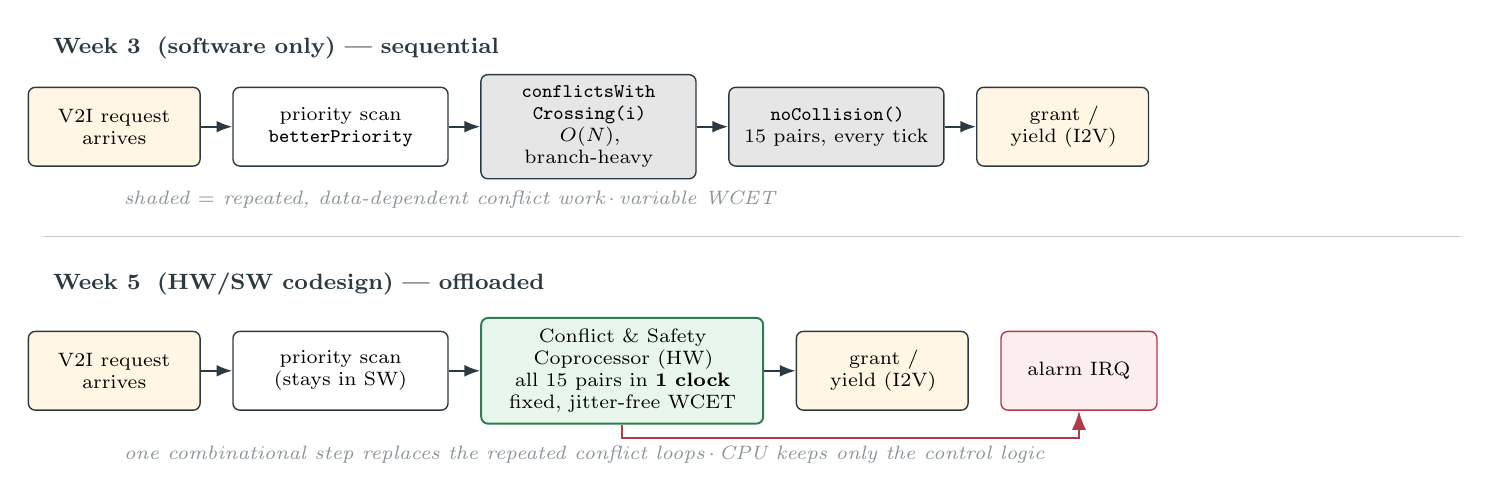
\begin{tikzpicture}[font=\footnotesize,node distance=4mm]

\tikzset{
  stg/.style={draw=ink,rounded corners=2.5pt,align=center,inner sep=4pt,font=\scriptsize,
              minimum height=10mm,text width=2.45cm,line width=0.5pt,fill=white},
  shd/.style={stg,fill=shadegray},
  hot/.style={stg,fill=hwbg,draw=hwgreen,line width=0.7pt,text width=3.3cm},
  io/.style={stg,fill=swbg,text width=1.9cm},
  irq/.style={stg,fill=critbg,draw=critred,text width=1.7cm,font=\scriptsize},
  a/.style={-{Latex[length=2mm]},line width=0.7pt,draw=ink},
}

% ---- Week 3 lane
\node[font=\bfseries\footnotesize,text=ink,anchor=west] (l1) at (0,3.55) {Week 3 \;(software only) --- sequential};
\node[io] (w3a) at (0.9,2.55) {V2I request arrives};
\node[stg,right=of w3a] (w3b) {priority scan\\\code{betterPriority}};
\node[shd,right=of w3b] (w3c) {\code{conflictsWith}\\\code{Crossing(i)}\\$O(N)$, branch-heavy};
\node[shd,right=of w3c] (w3d) {\code{noCollision()}\\$15$ pairs, every tick};
\node[io,right=of w3d] (w3e) {grant / yield (I2V)};
\draw[a] (w3a)--(w3b); \draw[a] (w3b)--(w3c); \draw[a] (w3c)--(w3d); \draw[a] (w3d)--(w3e);
\node[sub,anchor=west] at (0.9,1.62) {shaded $=$ repeated, data-dependent conflict work\,$\cdot$\,variable WCET};

% ---- divider
\draw[softrule,line width=0.4pt] (0,1.15) -- (18.0,1.15);

% ---- Week 5 lane
\node[font=\bfseries\footnotesize,text=ink,anchor=west] (l2) at (0,0.55) {Week 5 \;(HW/SW codesign) --- offloaded};
\node[io] (w5a) at (0.9,-0.55) {V2I request arrives};
\node[stg,right=of w5a] (w5b) {priority scan\\(stays in SW)};
\node[hot,right=of w5b] (w5c) {Conflict \& Safety Coprocessor (HW)\\all $15$ pairs in \textbf{1 clock}\\fixed, jitter-free WCET};
\node[io,right=of w5c] (w5e) {grant / yield (I2V)};
\node[irq,right=of w5e] (w5f) {alarm IRQ};
\draw[a] (w5a)--(w5b); \draw[a] (w5b)--(w5c); \draw[a] (w5c)--(w5e);
\draw[flowred,line width=0.7pt] (w5c.south) |- ($(w5f.south)+(0,-0.35)$) -- (w5f.south);
\node[sub,anchor=west] at (0.9,-1.62) {one combinational step replaces the repeated conflict loops\,$\cdot$\,CPU keeps only the control logic};

\end{tikzpicture}}
\caption{One grant decision. The repeated $O(N)$ and $O(N^2)$ conflict evaluation from Week~3 (shaded)
collapses into a single combinational hardware step in Week~5; the software keeps only the irregular
control logic, and the coprocessor additionally drives the collision-alarm interrupt.}
\label{fig:grant}
\end{figure}

% ======================================================================
\section{HW/SW Interface}
Software and hardware communicate through a small set of memory-mapped registers. On a real Zynq or
Kria board this is an AXI4-Lite slave; in the ModelSim co-simulation it is a simple register bus. The
interface is kept deliberately minimal: \emph{write the state, latch, read the result}. Because the
conflict matrix is combinational, the answer is valid in the same bus access. \code{ST_ALARM} is wired
to an interrupt, so a safety violation is caught on its own, separately from the scheduling code.

\begin{table}[h]
\centering
\caption{Memory-mapped register interface between the FreeRTOS RSU task and the coprocessor.}
\label{tab:regs}
\small
\begin{tabular}{@{}llcl@{}}
\toprule
\textbf{Register} & \textbf{Dir} & \textbf{Width} & \textbf{Meaning} \\
\midrule
\code{STATE_VEH[i]} & W     & 6 bits & \code{origin}(2), \code{turn}(2), \code{emergency}(1), \code{crossing}(1) for vehicle $i$ \\
\code{MODE}         & W     & 1 bit  & \code{MM_MODE}: $0={}$M/M/1, $1={}$M/M/2 \\
\code{CAND}         & W     & 3 bits & candidate id to test for \code{safe_to_grant} \\
\code{CTRL}         & W     & 1 bit  & start / latch inputs (result valid in the same access) \\
\code{ST_SAFE}      & R     & 1 bit  & \code{safe_to_grant(CAND)} for the current state and \code{MODE} \\
\code{ST_NOCOL}     & R     & 1 bit  & \code{noCollision()} over the whole fleet \\
\code{ST_CWC}       & R     & $N$ bits & \code{conflictsWithCrossing[i]} bit-vector \\
\code{ST_ALARM}     & R/IRQ & 1 bit  & \code{collision_alarm} (latched safety violation) \\
\bottomrule
\end{tabular}
\end{table}

\noindent
For each decision the RSU task writes the current \code{STATE_VEH[]} and \code{MODE} once, then for each
candidate writes \code{CAND} and reads \code{ST_SAFE}. A single writer (the RSU task) mirroring state
before each decision keeps hardware and software from drifting.

% ======================================================================
\section{Construct-by-Construct Mapping}
Each part of the verified model has exactly one execution target, which preserves the well-defined
mapping from models that the brief requires.

\begin{table}[h]
\centering
\caption{HW/SW assignment of every model and code construct, with the reason.}
\label{tab:map}
\small
\begin{tabular}{@{}p{5.8cm} c p{7.4cm}@{}}
\toprule
\textbf{UPPAAL / C construct} & \textbf{Target} & \textbf{Reason} \\
\midrule
\code{conflict(a,b)} & \textbf{HW} & pure Boolean of static rules; $15$ cells in parallel \\
\code{conflictsWithCrossing(i)} & \textbf{HW} & $O(N)$ scan becomes an $N$-bit combinational vector \\
\code{noCollision()} & \textbf{HW} & $O(N^2)$ monitor every tick; one cycle plus alarm IRQ \\
\code{capacityAvailableFor(i)} & \textbf{HW}\,$+$\,SW & capacity compare folded into \code{safe_to_grant} \\
\code{priorityValue} / \code{betterPriority} & SW & orchestration; changes with the aging term \\
\code{existsBetterGrantable(i)} & SW & depends on the priority policy, kept flexible \\
\code{emergencyWaiting()} & SW & trivial scan; drives the I2V yield broadcast \\
\code{canGrant(i)} & SW & thin wrapper that calls \code{hw_safe_to_grant()} \\
\code{requestVehicle} / \code{grantVehicle} / \code{finishVehicle} & SW & state updates plus queue and message side effects \\
Vehicle FSM (5 locations) $+$ clock \code{x[i]} & SW & one FreeRTOS task per vehicle, with software timers \\
\code{RSU_Controller} (req/grant/leave/yield) & SW & RSU task plus FreeRTOS queues \\
channels \code{req}/\code{grant}/\code{leave}/\code{i2v_yield}/\code{v2v_*} & SW & message queues / task notifications \\
\bottomrule
\end{tabular}
\end{table}

% ======================================================================
\section{Extension: Fairness / Aging (fixing the V5 starvation)}
\label{sec:aging}
To stop V5 from starving, we add an aging term so that the longer a vehicle waits, the higher its
effective priority becomes. A per-vehicle counter \code{age[i]} increments every tick while
\code{waiting[i]} is true and resets when the vehicle is granted, and the comparison in
\code{betterPriority()} becomes
\[
\text{effectivePriority}(i)\;=\;\code{priorityValue}(i)\;-\;k\cdot\code{age}[i].
\]
Aging is small, stateful and policy-dependent, so it belongs in software inside \code{betterPriority()};
the hardware conflict check is untouched. Crucially, \textbf{aging never overrides safety}: emergency
exclusivity, the capacity limit and the V4/V5 mutual exclusion are still enforced by
\code{safe_to_grant}, so aging only re-orders which of the \emph{already-safe} candidates is chosen.
This raises the Week~3 guarantee from \emph{safety only} to \emph{bounded waiting}, which we add as a
new liveness query in Section~\ref{sec:verif}.

% ======================================================================
\section{Verification and Co-Simulation Plan (Week 5)}
\label{sec:verif}
The plan keeps the verified UPPAAL queries as the contract and checks both sides against them.
\begin{itemize}
  \item \textbf{Hardware (ModelSim)}: a VHDL testbench feeds the coprocessor with state vectors and
  compares \code{noCollision} and \code{safe_to_grant} against reference values taken from the Week~3 C
  run. The key vector is V4 (North-right) and V5 (South-left) both crossing, which must report a
  conflict.
  \item \textbf{Exhaustive check}: the input space is small ($6$ bits per vehicle over the few origin
  and turn values the fleet actually uses), so the hardware outputs can be compared against the C
  reference over \emph{all} reachable states, not just a sample.
  \item \textbf{Software (FreeRTOS)}: the FreeRTOS version must reproduce the Week~3 trace --- the
  M/M/2 overlap of V1 and V2, and the emergency case where V0 pre-empts after an I2V yield --- with the
  three safety invariants kept as run-time assertions.
  \item \textbf{Co-simulation}: the RSU task drives the coprocessor over the register interface; the
  test fails if \code{hw_safe_to_grant} ever disagrees with the C reference.
\end{itemize}

\begin{table}[h]
\centering
\caption{Verification correspondence for the codesign, with the new liveness query added by aging.}
\label{tab:verif}
\small
\begin{tabular}{@{}p{6.6cm} c p{6.6cm}@{}}
\toprule
\textbf{UPPAAL query} & \textbf{Checked where} & \textbf{Mechanism} \\
\midrule
\code{A[] not deadlock} & SW & cyclic schedule always has an enabled action \\
\code{A[] noCollision()} & HW $+$ SW & HW monitor every clock, plus SW assertion \\
\code{A[] crossingCount <= MM_MODE} & HW $+$ SW & capacity in \code{safe_to_grant}, plus SW assertion \\
\code{A[] not(crossing[4] && crossing[5])} & HW $+$ SW & conflict cell $(4,5)=1$, used as a regression vector \\
\code{E<> crossing[0]} & SW & emergency V0 is granted (log $+$ counter) \\
\code{E<> crossing[1] && crossing[2]} & SW & V1 and V2 cross together in M/M/2 \\
\code{waiting[5] --> crossing[5]} \emph{(new)} & SW & bounded waiting once aging is enabled \\
\bottomrule
\end{tabular}
\end{table}

% ======================================================================
\section{Week 5 Work Plan, Deliverables and Risks}

\subsection{Deliverables}
\begin{itemize}
  \item \textbf{SW}: the FreeRTOS implementation (vehicle tasks, RSU task, queues, timers, aging)
  reproducing the Week~3 behaviour.
  \item \textbf{HW}: a synthesisable VHDL Conflict \& Safety Coprocessor with a ModelSim testbench and
  the golden regression vectors.
  \item \textbf{Integration}: the register-interface driver plus a co-simulation demonstration, pushed
  to the repository.
  \item \textbf{Report}: a chapter documenting the partition, the interface and the verification
  results.
\end{itemize}

\subsection{Risks and mitigations}
\begin{table}[h]
\centering
\small
\begin{tabular}{@{}p{6.2cm} p{9.0cm}@{}}
\toprule
\textbf{Risk} & \textbf{Mitigation} \\
\midrule
HW/SW state drift (stale registers) & one writer (the RSU task) mirrors the state before each decision; a mutex guards the shared arrays \\
Interface overhead cancels the HW benefit & keep it combinational with a single-cycle register read; write the state once per tick \\
ModelSim setup or licensing & use the Intel/Quartus Prime ModelSim edition from the brief and start the testbench early \\
Aging breaks a safety invariant & aging only re-orders \emph{safe} candidates; safety stays gated by \code{safe_to_grant}; add the liveness query \\
Behaviour drifts from Week~3 & golden vectors and assertions tie both parts back to the verified C reference \\
\bottomrule
\end{tabular}
\end{table}

% ======================================================================
\section{Summary}
The proposed split preserves the verified contract while placing each part of the Week~3 core where it
fits best: the irregular, frequently-changed scheduling and messaging logic in software on FreeRTOS, and
the regular, parallel, safety-relevant conflict checking
(\code{conflict}, \code{conflictsWithCrossing}, \code{noCollision}) in a hardware \emph{Conflict \&
Safety Coprocessor} that returns one \code{safe_to_grant} bit and runs an independent collision monitor.
This yields a grant decision with constant, bounded timing, a second hardware check of
\code{A[] noCollision()}, and a lighter CPU load, while the aging term lifts the guarantee from
\emph{safety only} to \emph{bounded waiting}. Week~5 is therefore a focused implementation and
verification task in FreeRTOS and ModelSim.

\end{document}
